\documentclass[letterpaper,10pt]{article}

\usepackage[utf8]{inputenc}
\usepackage[spanish]{babel}
\usepackage{fontenc}
\usepackage[dvipdfmx]{graphicx}
\usepackage{bmpsize,wrapfig,xcolor}
\usepackage{fullpage}
\usepackage{amssymb}
\usepackage[hidelinks]{hyperref}

% Para evitar que se indente solo a cada rato
\setlength\parindent{0pt}

\begin{document}
	\begin{titlepage}

		\begin{wrapfigure}{R}{0.3\textwidth}
			
\includegraphics[width=0.3\textwidth]{logoFCFM.png}
		\end{wrapfigure}

		\noindent \phantom - % "Hax" para que quede alineada la imagen con el texto

		Universidad de Chile

		Facultad de Ciencias Físicas y Matemáticas

		Depto. de Ciencias de la Computación

		CC4102 - Diseño y Análisis de Algoritmos

		\vfill

		\begin{center}
			\begin{Huge}
				{\textbf{Tarea 2}}
			\end{Huge}
		\end{center}

		\vfill

		\begin{flushright}
			\begin{tabular}{lll}
				Integrantes	&:	& Rodrigo Delgado\\
						&	& Belisario Panay\\
						&	& Gabriel Sanhueza\\
				Profesor	&:	& Gonzalo Navarro\\
				Ayudantes	&:	& Sebastián Ferrada\\
						&	& Willy Maikowski\\
				Auxiliar	&:	& Jorge Bahamondes\\
			\end{tabular}
		\end{flushright}

	\end{titlepage}

	% % % % % % % % % % % % % % % % % % % % % % % % % % % % % % % % % % % % % % % % % % % % % % % % % % % % % % % % % % % % % % % % % % % % % % % % % % % % % % % % % % % % % % % % % %
	\newpage
	% % % % % % % % % % % % % % % % % % % % % % % % % % % % % % % % % % % % % % % % % % % % % % % % % % % % % % % % % % % % % % % % % % % % % % % % % % % % % % % % % % % % % % % % % %

	\tableofcontents

	% % % % % % % % % % % % % % % % % % % % % % % % % % % % % % % % % % % % % % % % % % % % % % % % % % % % % % % % % % % % % % % % % % % % % % % % % % % % % % % % % % % % % % % % % %
	\newpage
	% % % % % % % % % % % % % % % % % % % % % % % % % % % % % % % % % % % % % % % % % % % % % % % % % % % % % % % % % % % % % % % % % % % % % % % % % % % % % % % % % % % % % % % % % %

	\section{Introducción}

	Un \textit{suffix tree} es un \textit{trie} (Trie: Estructura ordenada en forma de árbol) comprimido, el cual contiene todos los sufijos de un texto dado como sus llaves, y sus posiciones en el
	texto como sus valores.

	En el presente informe se muestra el diseño, implementación y experimentación del algoritmo de Ukkonen, el cual es un algoritmo de orden lineal para la creación de Suffix Trees,
	formada por Nodos que poseen información interna y referencias a sus hijos.

	En particular el algoritmo de Ukkonen para un Suffix Tree almacena los sufijos de un string en forma de árbol, de modo que cada arco contiene los caracteres para formar una palabra, y
	agregando caracteres sucesivos hasta que el árbol está completo.
	Por tanto, al momento de buscar, si se llega a una hoja (nodo terminal) es porque se recorrieron los arcos necesarios para formar un sufijo.

	La idea de la tarea es que el algoritmo a desarrollar es \textit{on-line}, de orden lineal ($O(n)$) y con una implementación más sencilla con respecto a algoritmos similares (algoritmo de Weiner
	y algoritmo de McCreight).

	\subsection{Problema a resolver}

	Un algoritmo estándar de creación de Suffix Tree toma tiempo $O(n^3)$, mientras que el algoritmo de Ukkonen toma tiempo $O(n)$.
	El problema consiste en realizar los pasos necesarios para la buena implementación del algoritmo, ya que pequeños errores en código pueden producir un algoritmo de mayor orden de magnitud
	y con ello se falla en el objetivo.

	Los pasos para realizarlos estan detallados en el enunciado de la tarea y en el \textit{paper} de Esko Ukkonen, creador del algoritmo.

	\subsection{Hipótesis}

	Si bien es un algoritmo lineal, el algoritmo posee una constante que hace que el tiempo pueda crecer de manera rapida. Además, como el algoritmo será escrito en Java como lenguaje,
	la eficiencia del algoritmo se podría ver reducida, dado que el \textit{garbage collector} usa la CPU para realizar sus funciones. Se espera demostrar que la constante del algoritmo
	varía con respecto al largo por motivos externos al algoritmo, lo cual se puede demostrar si para números pequeños el algoritmo sí demuestra un comportamiento lineal.

	% % % % % % % % % % % % % % % % % % % % % % % % % % % % % % % % % % % % % % % % % % % % % % % % % % % % % % % % % % % % % % % % % % % % % % % % % % % % % % % % % % % % % % % % % %
	\newpage
	% % % % % % % % % % % % % % % % % % % % % % % % % % % % % % % % % % % % % % % % % % % % % % % % % % % % % % % % % % % % % % % % % % % % % % % % % % % % % % % % % % % % % % % % % %

	\section{Diseño Teórico}

	\subsection{Main}

	En Main se crea un archivo de \textit{logging} para registrar el tiempo de creación del Suffix Tree y los resultados de búsqueda, a partir de un texto leído desde el disco.
	En particular:
	\begin{itemize}
		\item El texto leído se preprocesa (se eliminan puntuaciones, espacios, saltos de línea y todo lo que no corresponda al \textit{regex} [a-ZA-Z]).
		\item Se crea el Suffix Tree usando el algoritmo de Ukkonen.
		\item Se registra el tiempo de creación.
		\item Se generan palabras aleatorias del texto, para buscarlas usando el Suffix Tree.
		\item Se registran los resultados de búsqueda.
	\end{itemize}

	\subsection{Ukkonen}

	Clase principal del algoritmo. Aquí se realiza la totalidad de la ejecución del algoritmo de Ukkonen.

	Posee 5 métodos auxiliares:
	\begin{itemize}
		\item run(): Crea el Suffix Tree correspondiente, usando los siguientes métodos auxiliares.
		\item getPath(char s, Node n): Retorna el camino desde el nodo n, con el caracter s.
		\item search(String suffix, Node root): Busca el String \textit{suffix} en el nodo \textit{root}
		\item getSuffixes(Node root, String suffix, int count): Método auxiliar para search. Busca recursivamente en los nodos por el sufijo \textit{suffix} usando
		el número \textit{count} (usado para los caminos).
		\item getLeafPath(Node n, int count): Retorna el camino a partir del nodo n, recorriendo \textit{count} nodos internos.
	\end{itemize}

	\subsection{Last}

	Esta clase es usada para mostrar el final de un camino.

	\subsection{Node}

	Esta clase se usa para almacenar la información correspondiente a cada sufijo. Puede ser o no ser una hoja. Es clase padre de \textit{InternalNode}.

	\subsection{InternalNode}

	Esta clase extiende de \textit{Node} para usarse como nodo interno (i.e., explícitamente \textbf{no es} una hoja).

	\subsection{TextPreprocessor}

	Esta clase recibe un texto como String y devuelve solamente los caracteres que coinciden con el \textit{regex} [a-zA-Z ]. El resto de los caracteres se eliminan
	(entre los cuales están los saltos de línea, las puntuaciones y los espacios)

	\subsection{Logger}

	Esta clase recibe un nombre de archivo y escribe los datos que se le entregan a dicho archivo. Sirve para registrar la información necesaria para generar los gráficos del informe.

	% % % % % % % % % % % % % % % % % % % % % % % % % % % % % % % % % % % % % % % % % % % % % % % % % % % % % % % % % % % % % % % % % % % % % % % % % % % % % % % % % % % % % % % % % %
	\newpage
	% % % % % % % % % % % % % % % % % % % % % % % % % % % % % % % % % % % % % % % % % % % % % % % % % % % % % % % % % % % % % % % % % % % % % % % % % % % % % % % % % % % % % % % % % %

	\section{Presentación de los Resultados}

	\subsection{Tiempo de Creación del Suffix Tree}

% 	// TODO: Mostrar cuanto se tarda en crear un suffix tree, para N = 2 ** 15..21 palabras (aprox).
	Los resultados para los tiempos de construcción del Suffix Tree usando nuestra implementación son los siguientes:

	\begin{center}
		\begin{tabular}{|c|c|}
			\hline
			Largo del texto & Tiempo de Construcción (mseg)\\
			\hline
			$2^{15}$ & 6\\
			\hline
			$2^{16}$ & 11\\
			\hline
			$2^{17}$ & 16\\
			\hline
			$2^{18}$ & 19\\
			\hline
			$2^{19}$ & 20\\
			\hline
			$2^{20}$ & 28\\
			\hline
			$2^{21}$ & 34\\
			\hline
			$2^{22}$ & 34\\
			\hline
			$2^{23}$ & 34\\
			\hline
			$2^{24}$ & 34\\
			\hline
			$2^{25}$ & 34\\
			\hline
		\end{tabular}
	\end{center}

	\begin{center}
		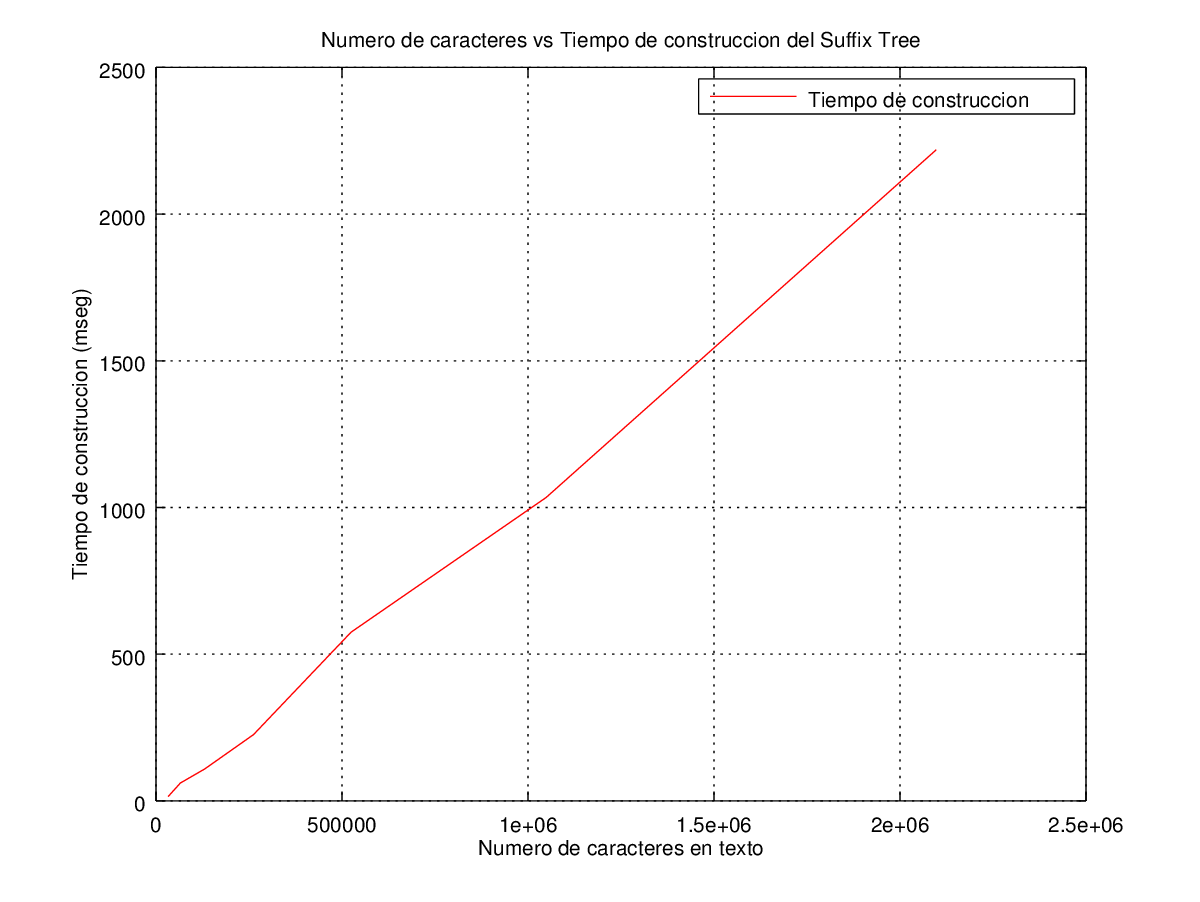
\includegraphics[width=0.8\textwidth]{fig1.png}

		Figura 1: Tiempo de creación del Suffix Tree para N = $2^{15..25}$
	\end{center}

	% % % % % % % % % % % % % % % % % % % % % % % % % % % % % % % % % % % % % % % % % % % % % % % % % % % % % % % % % % % % % % % % % % % % % % % % % % % % % % % % % % % % % % % % % %
	\newpage
	% % % % % % % % % % % % % % % % % % % % % % % % % % % % % % % % % % % % % % % % % % % % % % % % % % % % % % % % % % % % % % % % % % % % % % % % % % % % % % % % % % % % % % % % % %

	\subsection{Desempeño de operación \textit{Buscar}}

% 	// TODO: Mostrar cuanto se demora en buscar N = (2 ** 15..21) / 10 palabras (aprox).
	Los resultados para los tiempos de búsqueda en el Suffix Tree son los siguientes:

	\begin{center}
		\begin{tabular}{|c|c|c|}
			\hline
			Número de palabras & Largo promedio del patrón & Tiempo de búsqueda\\
			\hline
			$2^{15}$ & X & X\\
			\hline
			$2^{16}$ & X & X\\
			\hline
			$2^{17}$ & X & X\\
			\hline
			$2^{18}$ & X & X\\
			\hline
			$2^{19}$ & X & X\\
			\hline
			$2^{20}$ & X & X\\
			\hline
			$2^{21}$ & X & X\\
			\hline
			$2^{22}$ & X & X\\
			\hline
			$2^{23}$ & X & X\\
			\hline
			$2^{24}$ & X & X\\
			\hline
			$2^{25}$ & X & X\\
			\hline
		\end{tabular}
	\end{center}

	\begin{center}
		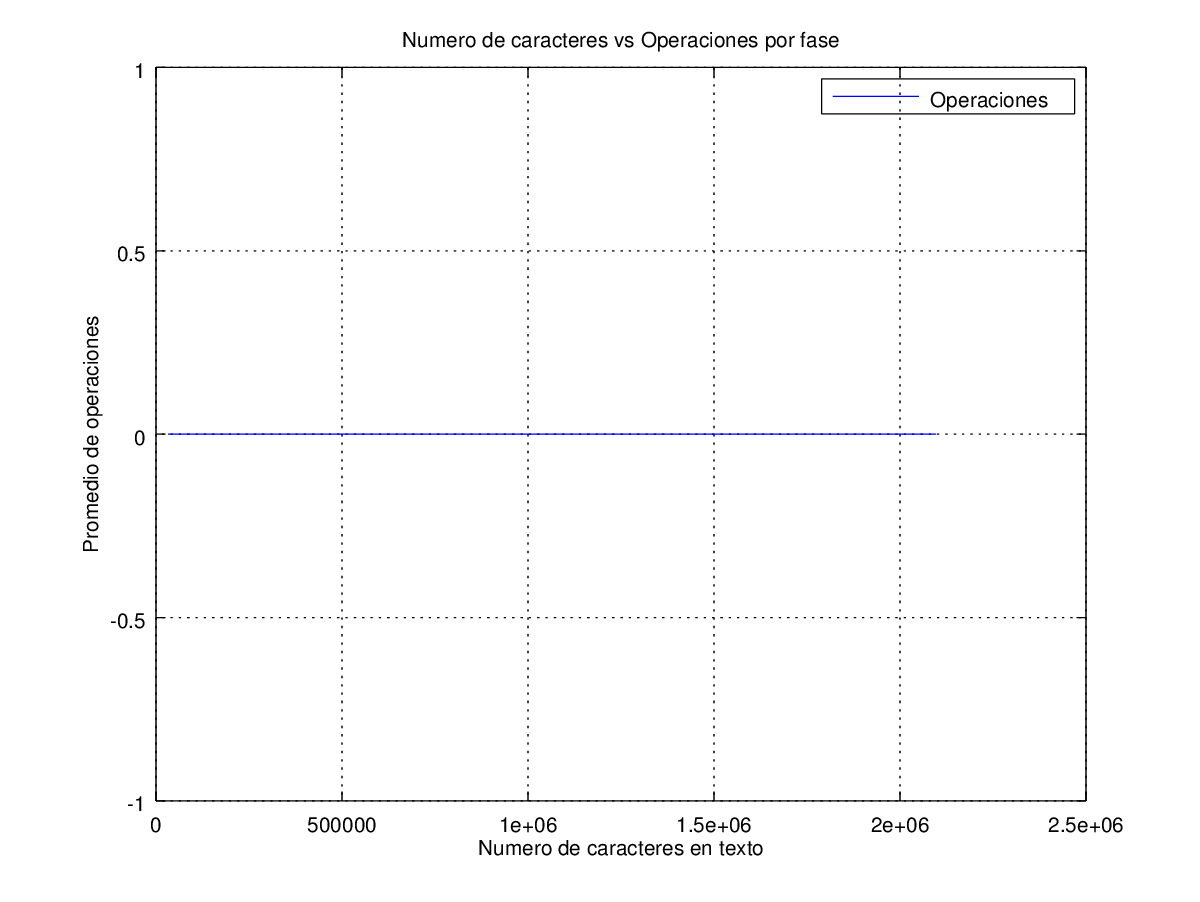
\includegraphics[width=0.8\textwidth]{fig2.png}

		Figura 2: Promedio de operaciones por fase
	\end{center}

	\begin{center}
		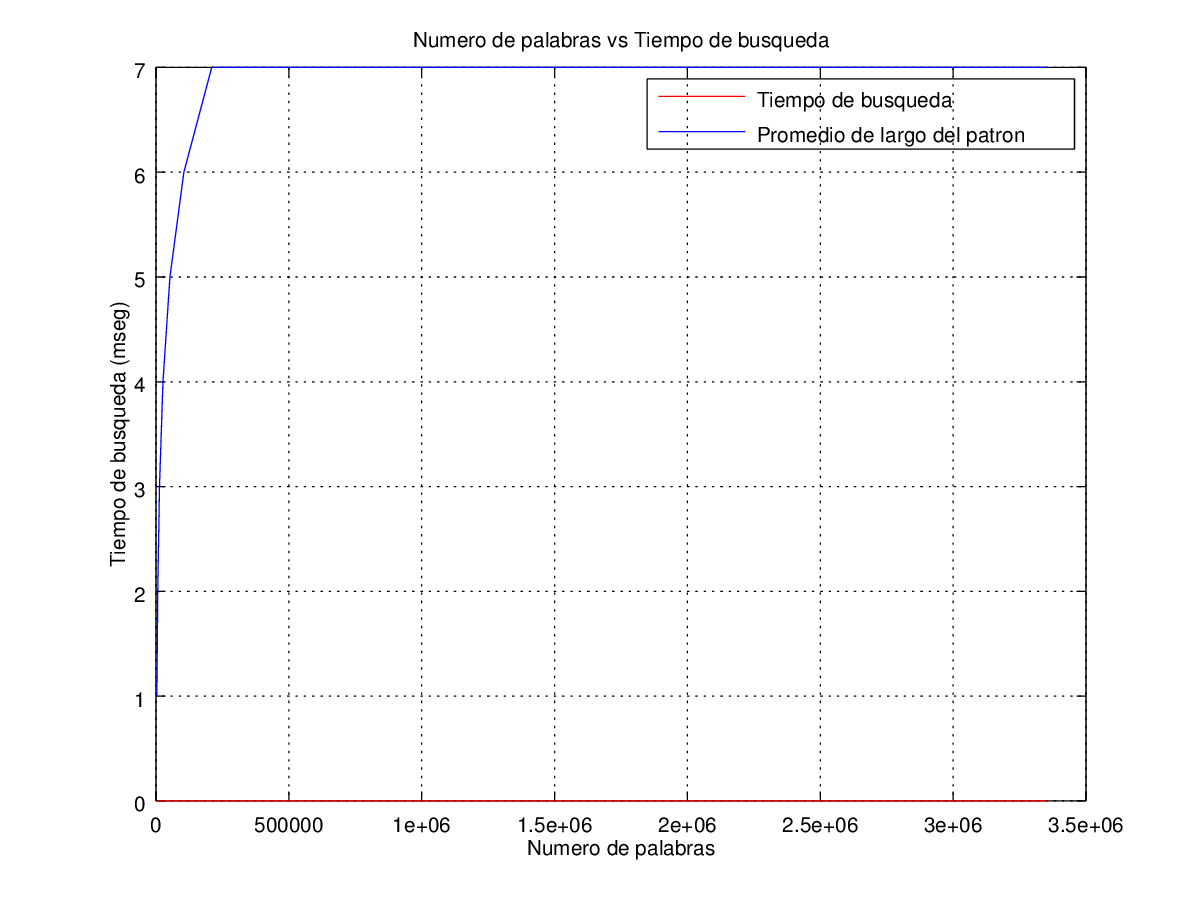
\includegraphics[width=0.8\textwidth]{fig3.png}

		Figura 3: Tiempo de búsqueda
	\end{center}

	% % % % % % % % % % % % % % % % % % % % % % % % % % % % % % % % % % % % % % % % % % % % % % % % % % % % % % % % % % % % % % % % % % % % % % % % % % % % % % % % % % % % % % % % % %
	\newpage
	% % % % % % % % % % % % % % % % % % % % % % % % % % % % % % % % % % % % % % % % % % % % % % % % % % % % % % % % % % % % % % % % % % % % % % % % % % % % % % % % % % % % % % % % % %

	\section{Análisis y Conclusiones}

	\subsection{Construcción del Suffix Tree}

% 	// TODO: Elegir versión de la conclusión

	% IF LINEAL
	Encontramos que el algoritmo de Ukkonen tarda X en N = $2^{15}$ caracteres, y se va duplicando (aproximadamente) cada vez que duplicamos la cantidad de caracteres, por lo que la
	implementación se consiguió hacer en tiempo $O(n)$.

	% IF INCONSISTENTE
	Además, nuestra hipótesis de que el \textit{garbage collector} de Java interferiría con nuestros resultados es correcta, dado que cada vez que se corría el algoritmo para una
	cantidad fija de caracteres variaba notablemente.

	% IF NOT DONE
	Nuestra implementación tuvo problemas al momento de ejecutarse, dado que no creaba correctamente los nodos internos. De esta forma el arbol se creaba demasiado rápido como para
	ser coherente con la cantidad de enlaces que deberían existir en el Suffix Tree.

	% IF ONLY WORDS
	Nuestra implementación funciona bien cuando se usan palabras cortas, dado que es posible construir el Suffix Tree en tiempo $O(n)$ (puesto que al duplicar el largo de la palabra,
	también se duplicaba el tiempo en nano-segundos para construirlo).

	\subsection{Búsqueda en el Suffix Tree}

% 	// TODO: Verificar si los tiempos están acotados o se fueron a la chu*** cada vez que aumentamos el número

	% IF TOO MUCH TIME
	Encontramos a partir de los resultados que la búsqueda se tarda más que la construcción del Suffix Tree. Probablemente se deba a problemas con la consistencia del árbol, dado que
	se espera que la búsqueda tome tiempo logarítmico respecto a la cantidad de caracteres en el texto.

	% IF GOOD
	Encontramos que la búsqueda toma tiempo logarítmico respecto a la cantidad de caracteres en el sufijo buscado. Esto se debe a que la estructura de árbol permite acelerar notablemente
	las búsquedas, además de que el Suffix Tree hace un \textit{tradeoff} entre tiempo y espacio ocupado.

	\subsection{Conclusiones}

% 	// TODO: Resumir lo ``aprendido'' (?)
% 	// TODO: Si no nos salió, explicar que podríamos hacer para arreglarlo (si tuvieramos más tiempo)

\end{document}
